\chapter{Results and discussion}

\textit{
In the previous chapter we described our main model and training procedure as well as some alternatives.
In this chapter we describe the numerical results of our implementation of the main model on two datasets, one synthetic dataset created from MNIST and the much more difficult Swedish population records. We also perform several experiments where we change the model configuration or training procedure and observe the effect on either or both datasets.
Hopefully, our observations can be instrumental in
% TODO: instrumental? Rephrase?
designing future encoder-decoder networks.
}

\section{Simulations on synthetic data}

Since the images of the Swedish records are so large, we decided to create a simpler and faster dataset so we could quickly iterate on the network architecture. Here we describe the synthetic dataset we created as well as some observations from altering the network configuration.

\subsection{Four-digit MNIST} \label{ssec:pretrain}


\begin{figure}
    \centering
    \begin{subfigure}[b]{0.45\textwidth}
        \centering
        
\includegraphics[scale=2.0]{resources/mnist4.jpg}
        \caption{Four digits without noise.
        %, size $112 \times 28$.
        }
        \label{fig:mnist4}
    \end{subfigure}%
    \begin{subfigure}[b]{0.45\textwidth}
        \centering
        
\includegraphics[scale=2.0]{resources/random_pad.jpg}
        \caption{Random position and dot noise.
        %Four digits with noise.
        %at a random position inside a box of $168 \times 56$ with dot noise.
        }
        \label{fig:mnist_random_pad}
    \end{subfigure}
    \caption{Two examples of generated synthetic data from MNIST.}
\end{figure}

For our early experiments we created a synthetic dataset with small images of four-digit sequences.
Each image was a concatenation of four independently randomly selected digit images from MNIST \cite{MNIST_orig}, where the first digit was always a one. See figure \ref{fig:mnist4} for an example. The resulting image was then a fixed size of $28 \times 112$ pixels.
%, compared to $900 \times 1500$ or more for the downsampled Swedish records.
% which is very much smaller than the images of the Swedish records.
Because the images were so small, it took a much shorter time to train and evaluate different models on the synthetic dataset than on the Swedish population records, whose images were very large.

Several models performed very well on this task, one of them achieving $94\%$ accuracy after 10,500 cpu-seconds of training. These models are discussed further in section \ref{sssec:exp_encoder}.

\subsection{Noisy MNIST}

In order to make the synthetic data a little bit more difficult to classify and more similar to the Swedish dataset, each four-digit image was placed at a random position in a larger image whose pixel values were zero, that is no ink.

When putting the four-digit image at a fixed position instead of a random position, one model learned to encode the distance from the left side of the image, which is quite interesting considering that neither the attention model nor the decoder had any explicit access to spatial information.
When adding $100$ additional zero-pixels to the right of the image, the accuracy dropped from $85\%$ to $80\%$. However, when adding $4$ zero-pixels to the left, the accuracy dropped to only $1\%$. We attribute this sudden accuracy loss to the difficulty of identifying which digit to keep and which to ignore. Since we are training on four-digit images but only expect the last three, the model must learn to find but ignore the first digit.
Since the year can appear at any position in the Swedish data, the simulations should also vary the position of the digits. Therefore, we must use random positions instead of fixed positions for the synthetic data.

Finally, we applied dot-noise to the image by:
(1) inverting the image so that the background is represented by one instead of zero,
(2) multiplying each pixel value with a random number drawn independently uniformly from $[0.6, 1.0]$ and
(3) inverting the image back again.
This corresponds to adding a random but small amount of ink to each pixel in the image.

An example image with dot noise and random position can be seen in figure \ref{fig:mnist_random_pad}. The models were evaluated on the image size $56 \times 168$ pixels, like in the figure.


\subsection{Network depth and width} \label{sssec:exp_encoder}


\begin{figure}
    \centering
    \begin{subfigure}[c]{1.0\textwidth}
        \centering    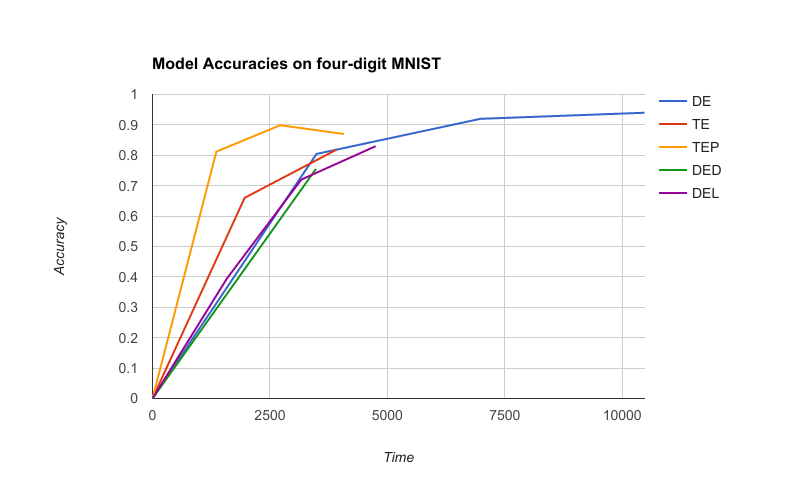
\includegraphics[scale=0.5]{resources/mnist_4_graph.png}
        \caption{Four-digit MNIST without noise.}
        \label{fig:mnist_early_models}
    \end{subfigure}
    \begin{subfigure}[c]{1.0\textwidth}
        \centering
        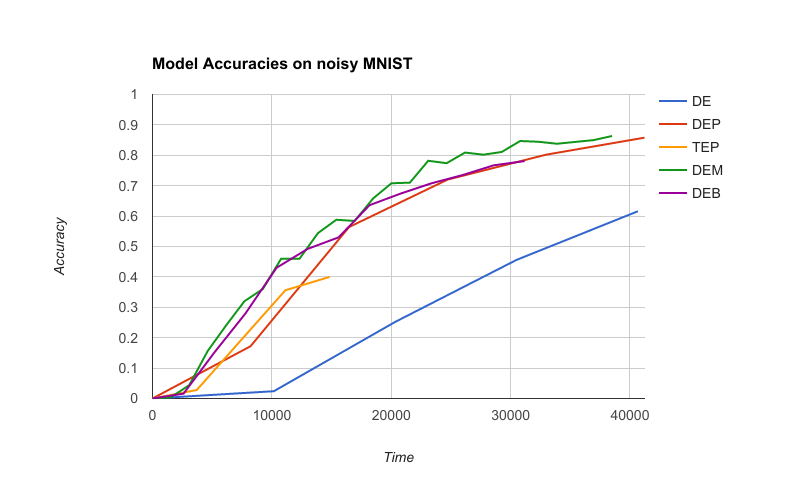
\includegraphics[scale=0.5]{resources/model_experiments.png}
        \caption{Noisy MNIST.}
        \label{fig:mnist_models}
    \end{subfigure}
    \caption{Plot of accuracy vs training time measured in CPU seconds for several models. Each data point comes after one epoch of training.}
\end{figure}


In figure \ref{fig:mnist_early_models} we can see the resulting accuracy over training time of some different model configurations.
All configurations used cartesian loss (defined in section \ref{sssec:cartesian}) and soft attention (see section \ref{sssec:soft_attention}).
The DE model was used as baseline with an encoder that had 7 layers and an output depth of 256. It is very similar to the DEP encoder illustrated in figure \ref{fig:encoder} except that it used one less pooling layer.

Halving the depth of the decoder from 1024 to 512 (DED) had little impact on this task. Halving the number of filters in every layer (DEL) halved the training time per epoch but also halved the learning rate, so in the end its performance was about the same.

% The TE model was identical to DE except that it used fewer convolutional layers. More precisely, the DE encoder started with $\langle C,C,P,C,C,P \rangle$ while TE started with $\langle C, P, C, P \rangle$, where $C$ stands for $3 \times 3$ convolution and $P$ stands for $2 \times 2$ max-pooling.

Reducing the number of convolutional layers in the beginning of the encoder (TE) also sped up training time although the accuracy over time was about the same.

When adding an additional pooling layer (TEP) to the thinner model (TE), learning increased very rapidly for the first two epochs. However, it started to overfit after hitting $90\%$ accuracy, while the accuracy of the baseline model (DE) continued to rise to $94\%$.

In summary we can see that models with smaller representational size achieves about the same accuracy given the same amount of training time, although the heavier models seem to have higher potential in the long run. Another observation is that additional pooling can greatly increase the early learning.

% The learning rate on the simpler four-digit MNIST dataset for different some possible configurations of the encoder.

% By training on the simpler four-digit MNIST dataset without noise,
%we made several observations.
% We experimented on various configurations of encoder and decoder depth and width.
% we found that increasing the width of the decoder's hidden layer from 512 to 1024 had a very small impact on the training time while increasing accuracy. Decreasing the number of layers in the encoder from 7 to 5 decreased the accuracy somewhat but increased training time considerably. Halving the encoder width halved the training time but also decreased accuracy. Adding a pooling layer at the end of the encoder resulted in a higher accuracy after the first epoch and reduced training time. The effect of an extra pooling layer can be seen by comparing the models TE and TEP in figure \ref{fig:mnist_early_models}.

\subsubsection{Wider networks are more robust to noise}

The best configurations so far were evaluated on the more difficult synthetic dataset with random positions and noise. Figure \ref{fig:mnist_models} contains a comparison between some variations of encoder configurations on the noisy MNIST dataset.
By comparing this graph to figure \ref{fig:mnist_early_models}, we can see that using larger input images, placing the digits at a random position and adding noise makes the problem much more difficult. Training a single epoch takes almost three times as long and the learning per epoch is reduced.
%Note that for the same model, we needed to train more than 4 times longer to get the same accuracy as on the simpler synthetic dataset.

The three best configurations (DEP, DEB, DEM) achieved very similar results considering the test accuracy vs training time. These three configurations had the same number of encoder layers but different depth of each layer.

The heaviest encoder (DEP) is illustrated in figure \ref{fig:encoder}.
Because it had the most number of filters, the training time for each epoch was much longer than for the other two alternatives.
% For this encoder the representational size of the input decreases exponentially for each pooling layer: 32, 16, 8, 4, 2.
Since each pooling layer divides the representational size by four and the number of filters in this model doubles after almost every pooling layer, the representational size decreases is halved after most pooling layers.

While the representational size decreases for DEP, as recommended by \textcite{InceptionV3}, the DEM encoder was designed to keep the representational size as constant as possible from the start.
This was done by reducing the number of filters to a minimal amount, with only 4 filters at the input layer instead of 32.
As we can see in figure \ref{fig:mnist_models}, the training time for each epoch was much faster although the actual learning over time was almost the same as for the DEP model.

The third competing encoder (DEB) was a middle ground between DEP and DEM, designed to have a very slowly decreasing representational size.


\begin{figure}
    \centering
    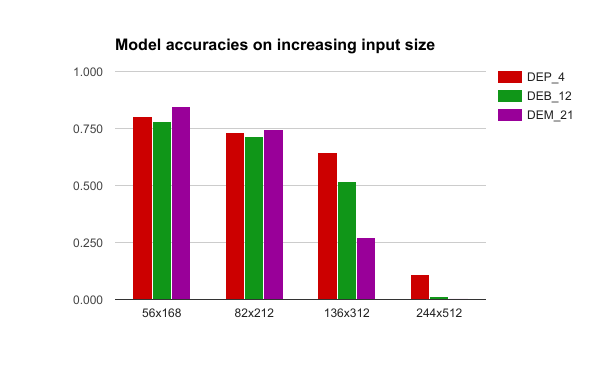
\includegraphics[scale=0.5]{resources/mnist_resilience.png}
    \caption{Noise resilience... TODO}
    \label{fig:mnist_resilience}
\end{figure}

When increasing the size of the generated synthetic images without retraining the models, the accuracy of the DEP model was relatively stable even for the double width and height but dropped for larger input. The two lighter models, DEB and DEM, were less robust to this change in input; see figure \ref{fig:mnist_resilience}.

The attention model is responsible for choosing the correct location in the input image. The receptive field of output units in the three configurations were the same and the architecture of the attention model was identical. The background noise was also identical. So although the attention model worked well for a smaller image, it is not sure it may work as well for a larger image where the background is the same.
% One possible reason for this is that the soft attention for all locations must sum to one. Since there are more locations to choose from, the weight on the correct location decreases.
Remember that the attention model does not know how many locations there are but outputs a salience score for each location independently. Since we use the softmax of these salience scores, the resulting attention weights must sum to one. So the more locations there are, the more the attention risk to spread out over noisy locations. To counter this, the attention model would have to be even more aggressive to separate background noise from useful signals. For hard attention however, only the most promising location is kept and the rest are ignored. So a model trained with hard attention should be more resilient to increased image size. We discuss more about attention later in section \ref{sssec:result_attention}.

We see that the more filters a model has, the more stable it is to change. Hence we believe that although on a single task the three configurations performed comparatively, the heavier model generalizes better in the long run.

% We attribute this resilience to noise to detecting more features in the input, some of which are better preserved after adding the noise.


% We argue that the heavier model, DEP, with its additional filters can detect more features in the input

% The lightest encoder (DEM) was designed to have the same representational size as DEP at the end of the encoder but decreasing the number of filters in the beginning in order
% keeping the representational size as constant as possible from the start by using fewer filters, in contrast to the advice from \textcite{InceptionV3}.


\section{Experiments} \label{sec:experiments}

In this section we present and discuss our model as well as some variations on the Swedish population records.
% metrics of different models and training
% comparisons we made between different models on the Swedish population records.

\subsection{Setup}


\subsubsection{Input}
The images of the Swedish population records had a high resolution so they were down sampled with a ratio of 8. So instead of having a size of $4688 \times 6360$ it was down sampled to $586 \times 795$. Because the images have different sizes, in each batch the images were padded with zeroes to get the same size as the largest image in the batch.

\subsubsection{Implementation}
The models were implemented in Tensorflow \cite{Tensorflow}, which is a popular open-sourced machine learning framework. The implementation\footnote{\url{https://github.com/HalfLeif/CNN_doc_extraction}} is freely available on Github.

\subsubsection{Hardware}
We trained the models on 3 threads on a single Intel(R) Core(TM) i7-4770K @ 3.50GHz. Training a single epoch of Swedish population records took about 28 hours. It would be faster to train using more threads or GPU acceleration but we were constrained by limited access to hardware.


\subsubsection{Pre-training}

All experiments in this section start with a pre-trained model already, we refer to this as the \textbf{base model}. The base model uses the DEP encoder and was trained using soft attention and cartesian loss for 5 epochs on the noisy MNIST and then for 16 epochs on the Swedish population data. Thus it had an accumulated training time of about 400,000 cpu-seconds.
% noisy MNIST DEP-5: 41217 cpusec
% 16 epochs of SweDEP: 22440*16 cpusec
% SUM: ca 400k cpusec.
The base model had a test accuracy of $8.39\%$ and an evaluation accuracy of $2.11\%$.

Optimally the experiment variations should be retrained from scratch, but since they are heavily pre-trained with another configuration, we present our observations as a lower bound to the potential accuracy of each variation.

% that pre-trained on the noisy MNIST for 5 epochs which was then trained on the Swedish population data

% The experiments in this section were performed after training the model for many epochs on the Swedish data already. Optimally we would want to retrain the model from scratch for each alteration but doing so would take too much time. Thus we can only provide a lower bound for the accuracy of the altered models.


\subsection{Independent digits} \label{sssec:ind_digits}

% TODO: check in notes for results on MNSIT data.



\subsection{Soft vs hard attention} \label{sssec:result_attention}

\textbf{TODO}: example image with soft and hard attention. Show both success and failure.

\subsection{Multi-year vs single-year loss function} \label{ssec:result_multiyear}

\section{Post-processing} \label{sec:result_post_process}

\section{Best model}

TODO: compare metrics and suggest best model. Also show confidence thresholds and other metrics.
